\documentclass[a4paper]{article}
\usepackage{a4wide}
\usepackage{tikz}
\usetikzlibrary{arrows,trees,automata}
\usepackage{aip}%             't beste als aip de laatste in de lijst is.

\usepackage{graphics}
\usepackage{graphicx}
\usepackage{pgf}
%\usepackage{palatino}
\usepackage{amsmath,amssymb}
\usepackage{bm}
\usepackage[english]{babel}
\usepackage{fancybox}
\usepackage{hyperref}

% colors
\def\red#1{{\color{red}#1}}
\def\blue#1{{\color{blue}#1}}
\definecolor{mygreen}{rgb}{0,.5,0}
\def\green#1{{\color{mygreen}#1}}

 % input, general variable
\newcommand{\xvar}{{X}}          % input variable X
\newcommand{\x}{{\mathit{x}}}    % scalar input x
\newcommand{\xv}{{\mathbf{x}}}   % (D x 1) vector input (\x_1, ...,\x_D)^T
\newcommand{\xmat}{{\mathbf{X}}} % (N x D) input matrix 
\newcommand{\xvec}{%             % (N x 1) input vector (N observations) 
	{\ensuremath{\boldsymbol{\mathsf{x}}}}}  
 
% target data
\newcommand{\yvar}{T}          %  target variable 
\newcommand{\y}{{\mathit{t}}}  %  scalar target value 
\newcommand{\yv}{{\mathbf{y}}} %  vector target
\newcommand{\yvec}{%           %  N x 1 target vector
	{\ensuremath{\boldsymbol{\mathsf{t}}}}} 

% latent variables
\newcommand{\zvar}{Z}            % latent variable 
\newcommand{\z}{{\mathit{z}}}    % latent var value 
\newcommand{\zv}{{\mathbf{z}}}   % K x 1 latent variable
\newcommand{\zmat}{{\mathbf{Z}}} % NxK latent var matrix 

% data sets
\newcommand{\data}{\mathcal{D}} % observed data set
\newcommand{\xset}{\{\xv_1,\dotsc,\xv_N\}} % input sequence
\newcommand{\yset}{\{\y_1,\dotsc,\y_N\}}   % target sequence
\newcommand{\xyset}{\{(\xv_1,\y_1),\dotsc,(\xv_N,\y_N)\}} % paired seq

% sequences (ordered sets)
\newcommand{\xseq}[2]{{\xv_{#1},\dotsc,\xv_{#2}}} 
\newcommand{\zseq}[2]{{\zv_{#1},\dotsc,\zv_{#2}}}

% other signals

\newcommand{\class}{{\mathcal{C}}} %  classes
\newcommand{\noise}{{\epsilon}} %  noise	
\newcommand{\noisevec}{%
	{\ensuremath{\boldsymbol{\epsilon}}}} 


%% parameters

\newcommand{\thpar}{{\theta}} % generic parameters
\newcommand{\thvec}{%
	{\ensuremath{\boldsymbol{\theta}}}}
\newcommand{\thold}{{\thvec^{\text{\red{old}}}}}
\newcommand{\thnew}{{\thvec^{\text{\red{new}}}}} 
\newcommand{\thlib}{{\Theta}}

\newcommand{\w}{{\mathit{w}}} % alternative parameter 
\newcommand{\wv}{{\mathbf{w}}} 
\newcommand{\wmat}{{\mathbf{W}}}
\newcommand{\wlib}{{\mathcal{W}}}

% prior
\newcommand{\prio}{{\pi}}
\newcommand{\priovec}{\ensuremath{\boldsymbol{\pi}}}

 % Gaussian pars

\newcommand{\Normal}{\mathcal{N}}
\newcommand{\Bern}{\mathrm{Bern}} % bernouilli

\newcommand{\mupar}{{\ensuremath{\mu}}}
\newcommand{\muvec}{{\ensuremath{\boldsymbol{\mu}}}}

\newcommand{\sgm}{{\sigma}}
\newcommand{\sgmsq}{{\sigma^2}}
\newcommand{\Sgm}{{\ensuremath{\boldsymbol{\Sigma}}}}
\newcommand{\Prec}{{\ensuremath{\boldsymbol{\Lambda}}}}


% prob, expectation, variance
\newcommand{\p}{p} % probability (mass and density)
\newcommand{\Exp}{\mathbb{E}} % expectation
\newcommand{\cov}{\mathrm{cov}} % covariance
\newcommand{\var}{\mathrm{var}} % variance

% chapter 12 on PCA

\newcommand{\vv}{{\mathbf{v}}}   % 
\newcommand{\vmat}{{\mathbf{V}}}   % 
\newcommand{\mv}{{\mathbf{m}}}   % 
\newcommand{\rmat}{{\mathbf{R}}}

% chapter 13 on PCA

\newcommand{\amat}{{\mathbf{A}}}   % 
\newcommand{\cmat}{{\mathbf{C}}} 
\newcommand{\Gambf}{{\ensuremath{\boldsymbol{\Gamma}}}}

% extra math
\newcommand{\realnumbers}{\mathbb{R}}
\newcommand{\beq}{\begin{equation}}
\newcommand{\eeq}{\end{equation}}

\newcommand{\trace}{\mathrm{Tr}}
\newcommand{\diag}{{\mathrm{diag}}}
\newcommand{\zerovec}{{\mathbf{0}}} % 0 vector
\newcommand{\llh}{{\mathit{L}}} % log likelihood
\newcommand{\resp}{\gamma} % responsibility
\newcommand{\Q}{\mathcal{Q}}  % expected complete llh
\newcommand{\KL}{\mathrm{KL}} % Kullback-Leibler divergence
\newcommand{\FreeEnergy}{\mathcal{L}}
\def\d#1{{\,\mathrm{d}#1}} % differential d in integrals
%\newcommand{\d}[1]{{\,\mathrm{d}#1}}





%%%
%%%
%%%

\newcommand{\A}{\mathcal{A}}
\newcommand{\B}{\mathcal{B}}
\newcommand{\C}{\mathcal{C}}
\newcommand{\D}{\mathcal{D}}
\newcommand{\E}{\mathcal{E}}
\newcommand{\I}{\mathcal{I}}
\newcommand{\M}{\mathcal{M}}
\newcommand{\N}{\mathcal{N}}
\newcommand{\X}{\mathcal{X}}
\newcommand{\Y}{\mathcal{Y}}
\newcommand{\mc}[1]{\mathcal{#1}}


% full page graph inclusion 
\newcommand{\incgraph}[1]{\includegraphics[keepaspectratio,width=\textwidth, height=.8\textheight]{#1}}





%colors
%\def\r#1{{\color{red}#1}}
%\def\b#1{{\color{blue}#1}}
%\definecolor{mygreen}{rgb}{0,.5,0}
%\def\g#1{{\color{mygreen}#1}}


\newcommand{\tjboxed}[1]{\par\begin{center}\tikz \node[draw,text width=13cm,inner sep=3pt,line width=1pt] {\parbox{13cm}{#1}};\end{center}}
%\newcommand{\tjboxed}[1]{}



%                        HEADER INFORMATIE
\examendatum{20 June 2011}                     % Datum van het examen.
\examentijd{14u00--17u00}                      % Tijd van het examen.

\begin{document}

\begin{exam}
%
% algemene vorm van invoer:
% gebruik het 'environment'
%       \begin{vraag}{xxx}
%         ...
%       \end{vraag}
% Hierin wordt in xxx beschreven hoe de verschillende onderdelen
% scoren. Per vraag zijn 10 punten te verdelen. Bij het nakijken per
% onderdeel een geheel aantal punten tussen 0 en aangegeven aantal
% toekennen.
%
% Deelvragen worden aangegeven door het environment
% \begin{deelvraag}
%   ...
% \end{deelvraag}
%

%%%
%%% Hier is vraag 1
%%%


\begin{vraag}{a) 2 points; b) 2 points; c)  1 point; d) 1 point; e) 3 points (total: 9)}
\mbox{}
\begin{deelvraag} 
Consider a data set $\data = \xset$ where we assume that each sample $\xv_n$ is IID distributed by a multivariate Gaussian (MVG), $\N(\xv_n|\,\muvec,\Sigma)$. 
Proof that the maximum likelihood estimate (MLE) of the mean value of this distribution is given by
\begin{equation}
\hat \muvec = \frac{1}{N}\sum_n \xv_n 
\label{eq:mvg-mu} 
\end{equation}

\tjboxed{  
\begin{align*}
\nabla_\mu \log \p(\data|\thvec) &= -\frac{1}{2}\sum_n \nabla_\mu \left[ (\xv_n-\muvec)^T \Sgm^{-1} (\xv_n-\muvec) \right] \notag \\
&= -\frac{1}{2}\sum_n \nabla_\mu \trace \left[ -2\muvec^T\Sgm^{-1}\xv_n + \muvec^T\Sgm^{-1}\muvec \right] \notag \\
&= -\frac{1}{2}\sum_n \left( -2\Sgm^{-1}\xv_n + 2\Sgm^{-1}\muvec \right) \notag \\
&= \Sgm^{-1}\,\sum_n \left( \xv_n-\muvec \right)
\end{align*}
Set to zero yields
$$
\hat \muvec = \frac{1}{N} \sum_n \xv_n
$$
} % end tjboxed
\end{deelvraag}

\begin{deelvraag}
Consider now a data set $\data = \xyset$ with 1-of-$K$ notation for the discrete classes, i.e.,
$$
\y_{nk} = \begin{cases} 1 & \text{if $\y_n$ in class $\class_k$}\\
        0 & \text{else} \end{cases}
$$
together with class-conditional distribution $p(\xv|\class_k,\thvec) = \N(\xv|\muvec_k,\Sgm)$ and multinomial prior $p(\class_k|\priovec) = \prio_k$.

Proof that the joint log-likelihood is given by
$$
\log \p(\data|\thvec) =  \sum_{n,k} \y_{nk} \log \N(\xv_n|\muvec_k,\Sgm) + \sum_{n,k} \y_{nk} \log \prio_k
$$
\tjboxed{
 \begin{align*}
 \log p(\data|\thvec) &= \sum_n \log \red{\prod_k} p(\xv_n,\red{\y_{nk}}|\thvec)^\red{{\y_{nk}}} =  \sum_{n,k} \y_{nk} \log  \blue{p(\xv_n,\y_{nk}|\thvec)}\\
     &=  \sum_{n,k} \y_{nk} \log \blue{\N(\xv_n|\muvec_k,\Sgm)} + \sum_{n,k} \y_{nk} \log \blue{\prio_k}
 \end{align*}
}%end tjboxed
\end{deelvraag}

\begin{deelvraag}
Show now that the MLE of the \emph{class-conditional} mean is given by
\begin{equation}\label{eq:clas-mu}
 \hat \muvec_k = \frac{\sum_n \y_{nk} \xv_n}{\sum_n \y_{nk}} 
\end{equation}
\tjboxed{  see lecture notes. } % end tjboxed
\end{deelvraag}

\begin{deelvraag}
Explain this formula (eqn 2) in relation to eqn 1,  the MLE for the mean of a MVG.
\tjboxed{Eqn 2 computes the sample proportion, just like eqn 1 , but now only for samples from class $k$. 
} % end tjboxed
\end{deelvraag}

\begin{deelvraag}
In the lecture notes, we also discussed the MLE for a \emph{clustering} problem and derived (for the $i$-th iteration of the EM algorithm):
\begin{equation}
\hat \muvec_k^{(i)} = \frac{\sum_n \resp_{nk}^{(i)} \xv_n}{\sum_n \resp_{nk}^{(i)}}
\label{eq:clus-mu}
\end{equation}
(i) What does $\resp_{nk}^{(i)}$ represent?\\
(ii) Express $\resp_{nk}^{(i)}$ in terms of $\z_{nk}$  and $\xv_n$\\
(iii) Why the iterative EM algorithm? 
\tjboxed{
(1) The responsibilty $\resp_{nk}^{(i)} = \Exp[\z_{nk}|\xv_n,\thvec^{(i-1)}]$ is a \emph{soft} class indicator.\\ (2) It is our best estimate of the binary class indicator $\y_{nk}$, given the input $\xv_n$.\\ (3) We need the iterative EM algorithm because in clustering we don't have a one-step solution to the maximum likelihood estimation problem.
} % end tjboxed
\end{deelvraag}

\end{vraag}




%%%
%%% Hier is vraag 2
%%%

\begin{vraag}{a) 1 point; b) 2 point; c) 1 point; d) 1 point; e) 2 points  (total: 7)}
Consider an \textrm{IID} data set $D=\{(x_1,y_1),\ldots,(x_N,y_N)\}$. We will model this data set by a model $y_n =\theta^T  f(x_n) + e_n$, where $f(x_n)$ is an $M$-dimensional feature vector of input $x_n$;  $y_n$ is a scalar output and  $e_n \sim \mathcal{N}(0,\sigma^2)$. (Note the list of formula's at the final page of this exam).  

\begin{deelvraag}
Rewrite the model in matrix form by lumping input features in a matrix $F=[f(x_1),\ldots,f(x_N)]^T$, outputs and noise in the vectors $y=[y_1,\ldots,y_N]^T$ and $e=[e_1,\ldots,e_N]^T$, respectively. 
\tjboxed{
 $y = F\theta + e$
} % end tjboxed
\end{deelvraag}

\begin{deelvraag}
Now derive an expression for the log-likelihood $\log p(y|\,F,\theta,\sigma^2)$.
\tjboxed{
\begin{align*}
\log p(D|\theta,\sigma^2) &= \log \N(y|\,F\theta ,\sigma^2)\\
    &\propto  -\frac{1}{2\sigma^2}\left( {y - F\theta } \right)^T \left( {y - F\theta } \right)
\end{align*}
} % end tjboxed
\end{deelvraag}

\begin{deelvraag}
Proof that the maximum likelihood estimate for the parameters is given by 
$$\hat\theta_{ml} = (F^TF)^{-1}F^Ty$$

\tjboxed{
Taking the derivative to $\theta$
$$
\nabla_\theta \log p(D|\theta) = \frac{1}{\sigma^2} F^T(y-F\theta)
$$
Set derivative to zero for maximum likelihood estimate
$$
\hat\theta = (F^TF)^{-1}F^Ty
$$
} % end tjboxed
\end{deelvraag}

\begin{deelvraag}
What is the predicted output value $y_\text{new}$, given an observation $x_\text{new}$ and the maximum likelihood parameters $\hat \theta_{ml}$. Work this expression out in terms of $F$, $y$ and $f(x_\text{new})$. 
\tjboxed{
 Prediction of new data point: $\hat y_{\text{new}} = \hat \theta^T f(x_\text{new}) = [(F^TF)^{-1}F^Ty]^T  f(x_\text{new}) $
} % end tjboxed
\end{deelvraag}

\begin{deelvraag}
Suppose that, before the data set $D$ was observed, we had reason to assume a prior distribution $p(\theta)=\N(0,\sigma_0^2)$. Derive the Maximum a posteriori (MAP) estimate $\hat \theta_{map}$.(hint: work this out in the $\log$ domain.)
\tjboxed{
 \begin{align*}
\log p(\theta|D) &\propto \log p(D|\theta) p(\theta) \\
    &\propto  -\frac{1}{2\sigma^2}\left( {y - F\theta } \right)^T \left( {y - F\theta } \right) + \frac{1}{2 \sigma_0^2}\theta^T \theta
\end{align*}
Derivative $\nabla_\theta \log p(\theta|D) = -\frac{1}{\sigma^2}F^T(y-F\theta) + (1/ \sigma_0^2) \theta$\\
Set derivative to zero for MAP estimate leads to 
$$\hat\theta_{MAP} = (F^TF + \frac{\sigma^2}{\sigma_0^2} I)^{-1}F^Ty$$
} % end tjboxed
\end{deelvraag}

\end{vraag} %2


% Hier is vraag 3
\begin{vraag}{each sub-question a through d: 1 point (total: 4)}
\mbox{}
\begin{deelvraag}
(a) Why is Principal Components Analysis more popular than Factor Analysis in signal and image processing applications?\\
(b) What is the difference between supervised and unsupervised learning?\\
\tjboxed{(Alternative answers may also be accepted)\\
(a) In signal and image processing, the components of a vector are often shifted (delayed) samples. In that case the noise variances are not affected, which is modeled correctly by PCA. \\ 
(b) In supervised learning concerns learning a map from inputs to targets. Unsupervised learning concerns analysis of data without targets, such as pattern discovery and compression.
} % end tjboxed
Mark the following two statements with a \textrm{TRUE} or \textrm{FALSE} flag.\\
\\
(c) If $X$ and $Y$ are independent Gaussian distributed variables, then $Z = 3X+Y$ is also a Gaussian distributed variable.\\
(d) The sum of two Gaussian functions is always also a Gaussian function.

\tjboxed{
(c) T, (d) F
} % end tjboxed
  \end{deelvraag}
\end{vraag}

%%%%%%%%%%%%%%%%
%%%
%%% MDL vragen
%%%

%%%%%%%%%%%%%%%%
%%%
%%% Vraag 4 
%%%

\newcommand{\xsum}{\ensuremath{\mathcal X}}
\newcommand{\xn}{\ensuremath{x^n}}
\renewcommand{\M}{\ensuremath{\mathcal M}}
\renewcommand{\B}{\ensuremath{\mu}}
\newcommand{\Bml}{\ensuremath{\hat{\B}_{ML}}}
\newcommand{\Nc}[1]{\ensuremath{N(#1|\xn)}}
%
\begin{vraag}{a) 3 points; b) 2 points; c) 1 point; d) 1 point; e) 3 points. Total 10 points}
    Consider a sequence \xn{} generated by an exponential model
    \M{} with an unknown parameter \B. So
    \begin{align*}
      p(x|\M,\B) &= \frac{1}{\B}e^{-x/\B},\quad\text{for a single symbol $x$,} \\
      \intertext{and thus}
      p(\xn|\M,\B) &= \frac{1}{\B^n}\prod_{i=1}^ne^{-x_i/\B},\quad\text{for a sequence $\xn$.}
    \end{align*}

\begin{deelvraag}
Derive an expression for the log-likelihood $\ell(\mu)\equiv \log p(\xn|\M,\B)$ 
as a function of the average value $\bar x = (1/n)\sum_{i=1}^n x_i$.
\tjboxed{%
\begin{align*}
\ell(\mu) &= \log \prod_i p(x_i|\M,\mu) = \sum_i \log \left(\frac{1}{\mu} e^{-x_i/\mu}\right) \\
    &= -n \log \mu - (1/\mu)\sum_i x_i \\
    &= -n \left( \log \mu + \bar{x}/\mu \right)
\end{align*}
where $\bar x = (1/n)\sum_{i=1}^N x_i$.
}
\end{deelvraag}

\begin{deelvraag}
What is the maximum likelihood estimate, $\Bml$, for $\mu$ based on
observations $\xn$?
\tjboxed{%
Set $\frac{\partial \ell}{\partial \mu} = -n \left(\frac{1}{\mu}
-\bar{x}/\mu^2 \right)$ to zero to get $ \Bml = \bar x$
(the sample mean).
}
\end{deelvraag}

\begin{deelvraag}
Let your observations be
\begin{align}
  x^{15} = (&0.7578,0.2808,3.4246,0.1069,0.6905,0.9240,0.2466,0.7749, \nonumber \\
            &3.1880,0.5657,0.6044,2.2380,1.8625,0.2467,2.6036).
\end{align}
So $\sum_{i=1}^{15}x_i= 18.5161$. Determine the ML
      estimate \Bml{} in this case.
      \tjboxed{%
        In this case $n=15$ and $\sum_{i=1}^{15}x_i= 18.5161$, so
        \[ \Bml = 1.2344. \]
      }
\end{deelvraag}
\begin{deelvraag}
      Also, derive an expression for the ML sequence probability
      $p(x^{15}|\M,\Bml)$ for $x^{15}$ as given in equation~4.
      \tjboxed{%
      	We denote $\sum_{i=1}^{15}x_i= 18.5161$ by $\xsum$.\newline
        Straightforward, just plug-in \Bml{} into the given
        expression, so
        \begin{align*}
          p(\xn|\M,\Bml) &= \frac{1}{\Bml^n}\prod_{i=1}^ne^{-x_i/\Bml} \\
          &= \left(\frac{n}{\xsum}\right)^n e^{-n}. \\
          \intertext{Actually, a numerical answer is also fine.}
          &= 1.2993\cdot10^{-8}
        \end{align*}
      }
\end{deelvraag}
\begin{deelvraag}
    You are now given a \emph{prior} over \B, namely
      \[
      p(\B|\M) = \begin{cases}
        1; \text{if } \B\in[1,2], \\
        0; \text{if } \B\not\in[1,2].
      \end{cases}
      \]
      Derive the Laplace approximation of
      \[ p(x^{15}|\M) = \int_0^{\infty} p(\B|\M)p(x^{15}|\M,\B) \,d\B, \]
      where $x^{15}$ is again as given in equation~4.
      \tjboxed{%
		Consider $$f(\B)=p(\xn|\M,\B).$$ We know from (4) that it has a maximum at $$\Bml=1.2344$$ which
		lies in the valid range for $p(\B|\M)$. So we must evaluate the second derivative of $\ln f(\B)$
		in $\Bml$.      
		\newline
        \begin{align*}
          \ln f(\B) &= -15\ln \B - \frac{\xsum}{\B}. \\
          \frac{\partial \ln f}{\partial\B} &= \frac{-15}{\B}+\frac{\xsum}{\B^2}. \\
          \frac{\partial^2 \ln f}{\partial\B^2} &=
          \frac{15}{\B^2}-\frac{2\xsum}{\B^3} \\
          \frac{\partial^2 \ln f(\Bml)}{\partial\B^2} &=
          -\frac{15^3}{\xsum^2} < 0.
        \end{align*}
        Then the Gaussian approximation is
        \begin{align*}
          g(\B) &= \left(\frac{n}{\xsum}\right)^n e^{-n}
          \exp\left(-\frac12(\B-\frac{\xsum}{n})^2
            \frac{n^3}{\xsum^2}\right) \\
          &= \left(\frac{n}{\xsum}\right)^n
          e^{-n(1+(\frac{n}{\xsum}\B-1)^2))}
        \end{align*}
        The integral of $g(\B)$ gives
        \begin{align*}
          \int g(\B)\,d\B &= \sqrt{\frac{2\pi}{n^3}}\xsum
          \left(\frac{n}{\xsum}\right)^n e^{-n} \\
          &= 1.0380\cdot10^{-8}\text{ for the given sequence}.
        \end{align*}
        We show a plot of $p(\B|\M)p(x^{15}|\M,\B)$ and $g$, both
        as a function of $\B$.
        \begin{center}
            \includegraphics{laplaceApprox.pdf}
        \end{center}
      }
\end{deelvraag}
\end{vraag}

%%%
%%% Einde vraag 4

%%%%%%%%%%%%%%%%%%%%%%
%%%
%%% vraag 5
%%%

\renewcommand{\M}{\ensuremath{S}}
\newcommand{\cS}{\ensuremath{\mathcal S}}
\newcommand{\pt}{\ensuremath{\theta}}

\begin{vraag}{a) 5 points; b) 5 points. Total 10 points}
  We observe a binary sequence $x^{15}=110\,111\,101\,100\,001$. (The
  spacing is just for ease of reading and has no other meaning.)
  Assume that this sequence is preceded by two zeros as the initial
  context.

  Consider a context model \cS{} of depth 2 and the ``CTW prior''
  $P(\M_i)$ given as:
    \begin{align*}
      \Delta_2(\M) &= 2|\M|-1-|\{s\in\M: |s|=2\}|, \\
      P(\M_i) &= 2^{-\Delta_2(\M_i)}
    \end{align*}

  The following five tree structures are possible models, $\M_0$,
  $\M_1$, $\M_2$, $\M_3$, and
  $\M_4$:

  \noindent\hspace*{-1.5cm}
  \begin{center}
    \begin{tabular}{c@{\qquad}c@{\qquad}c@{\qquad}c@{\qquad}c}
      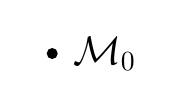
\begin{tikzpicture}
        \fill (0,0) circle (0.7mm) node[left=2pt] {$\pt$} node[right=4pt] {\Large$\M_0$};
      \end{tikzpicture}
      &
      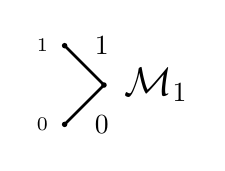
\begin{tikzpicture}[scale=0.5]
        \fill (0,0) circle (0.7mm) node[right=4pt] {\Large$\M_1$};
        \fill (-1,1) circle (0.7mm) node[left=2pt] {$\pt_1$};
        \fill (-1,-1) circle (0.7mm) node[left=2pt] {$\pt_0$};
        \draw[line width=1pt] (-1,1) -- node[above right] {$1$} (0,0)
          -- node[below right] {$0$} (-1,-1);
      \end{tikzpicture}
      &
      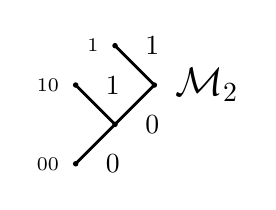
\begin{tikzpicture}[scale=0.5]
        \fill (0,0) circle (0.7mm) node[right=4pt] {\Large$\M_2$};
        \fill (-1,1) circle (0.7mm) node[left=2pt] {$\pt_1$};
        \fill (-1,-1) circle (0.7mm);
        \fill (-2,0) circle (0.7mm) node[left=2pt] {$\pt_{10}$};
        \fill (-2,-2) circle (0.7mm) node[left=2pt] {$\pt_{00}$};
        \draw[line width=1pt] (-1,1) -- node[above right] {$1$} (0,0)
          -- node[below right] {$0$} (-1,-1) -- node[above right] {$1$} (-2,0);
        \draw[line width=1pt] (-1,-1) -- node[below right] {$0$} (-2,-2);
      \end{tikzpicture}
      &
      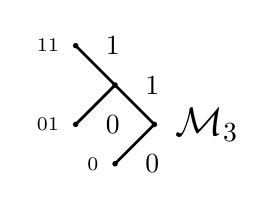
\begin{tikzpicture}[scale=0.5]
        \fill (0,0) circle (0.7mm) node[right=4pt] {\Large$\M_3$};
        \fill (-1,-1) circle (0.7mm) node[left=2pt] {$\pt_0$};
        \fill (-1,1) circle (0.7mm);
        \fill (-2,0) circle (0.7mm) node[left=2pt] {$\pt_{01}$};
        \fill (-2,2) circle (0.7mm) node[left=2pt] {$\pt_{11}$};
        \draw[line width=1pt] (-2,2) -- node[above right] {$1$} (-1,1)
          -- node[below right] {$0$} (-2,0);
        \draw[line width=1pt] (-1,1) -- node[above right] {$1$} (0,0) -- node[below right] {$0$} (-1,-1);
      \end{tikzpicture}
      &
      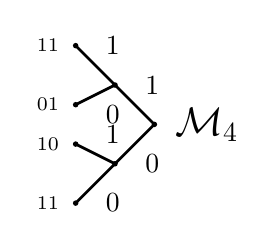
\begin{tikzpicture}[scale=0.5]
        \fill (0,0) circle (0.7mm) node[right=4pt] {\Large$\M_4$};
        \fill (-1,-1) circle (0.7mm);
        \fill (-1,1) circle (0.7mm);
        \fill (-2,2) circle (0.7mm) node[left=2pt] {$\pt_{11}$};
        \fill (-2,0.5) circle (0.7mm) node[left=2pt] {$\pt_{01}$};
        \fill (-2,-0.5) circle (0.7mm) node[left=2pt] {$\pt_{10}$};
        \fill (-2,-2) circle (0.7mm) node[left=2pt] {$\pt_{11}$};
        \draw[line width=1pt] (-2,2) -- node[above right] {$1$} (-1,1)
          -- node[below right] {$0$} (-2,0.5);
        \draw[line width=1pt] (-2,-2) -- node[below right] {$0$} (-1,-1)
          -- node[above right] {$1$} (-2,-0.5);
        \draw[line width=1pt] (-1,1) -- node[above right] {$1$} (0,0) -- node[below right] {$0$} (-1,-1);
      \end{tikzpicture}
    \end{tabular}
  \end{center}

  \begin{deelvraag}
    Compute the probability of this sequence in the recursive ``CTW'' manner.
    So, compute recursively
    \[ P^{\lambda}_w(x^{15})=\sum_{i=0}^4P(\M_i)P(x^{15}|\M_i). \]
    \tjboxed{%
      We consider a binary context tree of depth 2. We must collect
      the number of zeros and ones in eacht of the contexts
      $\lambda,0,1,00,10,01,$ and $11$. We find\\
      \[\begin{array}{c|rr}
        s  & N(s0|x^{15})=a & N(s1|x^{15})=b \\
        \hline
        \lambda & 6 & 9 \\
        0  & 3 & 4 \\
        1  & 3 & 5 \\
        00 & 2 & 2 \\
        10 & 1 & 2 \\
        01 & 0 & 3 \\
        11 & 3 & 2
      \end{array}\]
      From this we calculate the $P_e(a,b)$'s and the $P_w^s$'s.\\
      \[\begin{array}{c|ll}
        s  & P_e(a,b) & P_w^s \\
        \hline
        00 & 2.3438\cdot10^{-2}  &  2.3438\cdot10^{-2} \\
        10 & 6.25\cdot10^{-2}      &  6.25\cdot10^{-2} \\
        01 & 3.125\cdot10^{-1}     &  3.125\cdot10^{-1} \\
        11 & 1.1719\cdot10^{-2}   &  1.1719\cdot10^{-2} \\
        0  & 2.4414\cdot10^{-3}    & 1.9531\cdot10^{-3} \\
        1  & 1.3733\cdot10^{-3}     & 2.5177\cdot10^{-3} \\
        \lambda & 8.3596\cdot10^{-6} & 6.6347\cdot10^{-6}
      \end{array}\]
      The requested probability is $p_w^{\lambda}=6.6347\cdot10^{-6}$.
    }
  \end{deelvraag}

  \begin{deelvraag}
    Determine the a-posteriori model probabilities for these five
    models.
    \tjboxed{%
      For every model we must compute
      $2^{-\Delta_2(\M)}\prod_{s\in\M}P_e(a_s,b_s)/P_w^{\lambda}$.
      \[\begin{array}{clll}
        \M    & 2^{-\Delta_2(\M)} & P(x^{15}|\M) & P(\M|x^{15}) \\
        \M_0 & 2^{-1}                 & 8.3596\cdot10^{-6} & 0.630 \\
        \M_1 & 2^{-3}                 & 3.3528\cdot10^{-6} & 0.063 \\
        \M_2 & 2^{-3}                 & 2.0117\cdot10^{-6} & 0.038 \\
        \M_3 & 2^{-3}                 & 8.9407\cdot10^{-6} & 0.168 \\
        \M_4 & 2^{-3}                 & 5.3644\cdot10^{-6} & 0.101
      \end{array}\]
    }
  \end{deelvraag}
\end{vraag}

%%%%%%%%%%%%%%%%%%%%%%%%%%%%%%%%%%%%%%%%%%%%%%%%%%%
%%%
%%% APPENDICES
%%%


%
%\newpage
\vspace{1cm}\streep\vspace{1cm}
\section*{Appendix: formula's}
\begin{align*}
|A^{-1}|&=|A|^{-1} \\
\nabla_A \log |A| &= (A^{T})^{-1} = (A^{-1})^T \\
\trace[ABC]&= \trace[CAB] = \trace[BCA]  \\
\nabla_A \trace[AB] &=\nabla_A \trace[BA]= B^T  \\
\nabla_A \trace[ABA^T] &= A(B+B^T)\\
 \nabla_x x^TAx &= (A+A^T)x\\
\nabla_X a^TXb &= \nabla_X \trace[ba^TX] = ab^T
\end{align*}

\medskip
Multivariate gaussian
$$
\N(x|\,\mu,\Sigma) = |2 \pi \Sigma|^{-\frac{1}{2}} \exp\left\{-\frac{1}{2}(x-\mu)^T
\Sigma^{-1} (x-\mu) \right\}
$$

\end{exam}
\end{document}
